\subsection{Normalisation of simply typed linear $\lambda$-terms}
\label{sec:one-register}

% In this section, we explain how $\lambda$-terms can be evaluated using a derivable function, assuming that the $\lambda$-terms are linear and  can be typed using a bounded number of types. These notions will be explained in more detail below.  



We assume that the reader is familiar with the basic notions of the simply typed $\lambda$-calculus; more detailed definitions can be found in~\cite{sorensen_lectures_2006}. 
Define  \emph{simple types} to be expressions  generated from an atomic type $\otype$ using a binary arrow constructor, as in the following examples:
\begin{align*}
    \otype \qquad \otype \to \otype \qquad (\otype \to \otype) \to (\otype \to \otype) \qquad \cdots 
\end{align*}
In this paper,  the atomic type $\otype$ represents trees over the output alphabet.
Let $X$ be a set of variables, each one with an associated simple type.  A $\lambda$-term  is any expression that is constructed by starting with the variables, and using $\lambda$-abstraction $\lambda x. M$ and term application $M N$. 
We say that a $\lambda$-term is \emph{well-typed} if one can associate  to it  a simple type according to the usual typing rules of simply typed $\lambda$-calculus,
see~\cite[Definition 3.2.1]{sorensen_lectures_2006}. Because the variables are typed, a  $\lambda$-term has  either a unique type, or is not well-typed.  Here is an example of a well-typed $\lambda$-term, with the type annotation in blue: 
\begin{align*}
    \typecolor{\overbrace{
        \usualcolor{\lambda \typevar y {\otype \to \otype}. \ \lambda \typevar x \otype.}  \ \underbrace{\usualcolor{y (y x).}}_{\otype}}^{(\otype \to \otype) \to \otype \to \otype}}
    \end{align*}

% \footnote{
% Here we assume that the variables are typed, but the types for the remaining $\lambda$-terms need to be inferred. We could adopt a different approach, more thoroughly in the style of Church, where all term constructors (application and $\lambda$-abstraction) come decorated with the type of the resulting term. We do not do this to make  notation lighter, and also because one show -- see the appendix -- that first-order logic is enough to reconstruct the type of a term once the types of the variables are known. 
% }
    
% \begin{center}
% \includegraphics[scale=.3, page=45]{pics.pdf}
% \end{center}
We use the standard notion of $\beta$-reduction for $\lambda$-terms, see~\cite[Definition 1.2.1]{sorensen_lectures_2006}.  
Because of normalisation and confluence for the simply typed $\lambda$-calculus, every well-typed $\lambda$-term has a unique normal form, i.e~a $\lambda$-term to which it $\beta$-reduces (in zero or more steps), and which cannot be further $\beta$-reduced.

A $\lambda$-term  can be seen as a tree over the ranked alphabet
\begin{align}
    \label{eq:alphabet-for-lambda-terms}
  \overbrace{\set{x : x \in X}}^{\text{arity 0}} \cup \overbrace{\set{\lambda x : x \in X}}^{\text{arity 1}} \cup  \overbrace{\set @}^{\text{arity 2}}
\end{align}
where @ represents term application. Using this representation, and assuming that the set of variables is finite, it makes sense to talk about the tree-to-tree function
\begin{align*}
\text{$\lambda$-term} \qquad \mapsto \qquad \text{its normal form},
\end{align*}
which we call normalisation of $\lambda$ terms. 
 We show that this function is derivable, under two assumptions on the input $\lambda$-term. 
 
 The first assumption is that the input $\lambda$-term is \emph{linear}: 
    every bound variable is exactly once in its scope\footnote{This restriction could easily be relaxed to ``at most once''.}, but free variables are allowed to appear multiple times.  
    % If we allowed non-affine terms, then evaluation could lead to normal forms of super-linear size (e.g.~exponential), and thus could not be derivable.  For affine $\lambda$-terms, each step of $\beta$-reduction reduces the size by two or three, and therefore the normal form cannot be bigger than the original $\lambda$-term. 
     The second assumption is that  the input $\lambda$-term can be typed using a fixed finite set of types $\Tt$: it has type in $\Tt$, and the same is true for all of its  sub-terms.  In Appendix~\ref{sec:explaining-restrictions}, we explain why  assumptions are needed.


% Because of iterated duplication, the normal form of a well-typed $\lambda$-term can be exponential, as witnessed by Example~\ref{ex:exponential} in the appendix.
% Because derivable and first-order transductions have linear size increase, they cannot compute normal forms in general. To  avoid this problem, we  limit attention to affine $\lambda$-terms: a $\lambda$-term is called \emph{affine} if  

% Being affine alone is not enough to normalise terms with first-order transductions. Another obstacle is terms that use types of unbounded complexity, as illustrated by Example~\ref{ex:affine-not-enough} in the appendix.
% If the size of types that occur in subterms of our affine $\lambda$-terms is not bounded, and if we suppose that there is a first-order transduction which normalises them, then we could derive a first-order formula which performs an equality test between two integers Such a formula cannot exist (even if we allow monadic second-order logic).



% we define $\Lambda_\Tt X $ to be the set of affine $\lambda$-terms using variables from $X$, whose subterms have 	 types in $\typeset$.  When restricted to $\lambda$-terms of $\Lambda_\Tt X $, normalisation can be done by a derivable function, and therefore also by a first-order tree-to-tree transduction: 

\begin{theorem}\label{thm:normalise} Let $X$ be a finite set of simply typed variables, and let $\typeset$ be a finite set of simple types.
    The following tree-to-tree function is derivable, assuming that $\lambda$-terms are represented as trees:
    \begin{itemize}
        \item{\bf Input.} A $\lambda$-term over variables $X$.
        \item {\bf Output.} Its normal form, if it is linear and  can be typed using $\Tt$, and undefined otherwise.
    \end{itemize}
\end{theorem}

This is one of our main technical contributions, and its proof is in Appendix~\ref{sec:eval}. A key role in the proof is played by the pre-order function. 

% Actually, we prove a stronger result, namely that the above function is derivable. In the end, of course, we will prove that all first-order tree-to-tree transductions are derivable, but our proof of this fact will use the derivability of normalisation as stated in Theorem~\ref{thm:normalise}.



% Recall that elements of $\tmonad \rSigma$ are defined to be trees over $\rSigma + \varnames$, where 
% \begin{align*}
%     \varnames = \set{x_1,x_2,\ldots}
% \end{align*}
% is a fixed set of  variable names that are used for ports. In this section, we view $\varnames$ as a simply typed set, where all variables $x_1,x_2,\ldots$ have the same simple type $\otype$.  Under this convention, we can view
% \begin{align*}
%     \tmonad (\overbrace{\set{x : x \in X}}^{\text{arity 0}} \cup \overbrace{\set{\lambda x : x \in X}}^{\text{arity 1}} \cup  \overbrace{\set @}^{\text{arity 2}})
% \end{align*}
% as a set of $\lambda$-terms. This is exactly the set of those $\lambda$-terms over variables $X + \varnames$ where: (a) variables from $\varnames$ are never bound; and (b) there is some $n$ such that each of the variables $x_1,\ldots,x_n \in \varnames$  appears as a free variable exactly once  and the remaining variables in $\varnames$ do not appear at all. If $S$ is a finite set of simple types, then define  $\linterm S X$ to be those terms in .. which are linear and $S$-typed. 

% Computing the normal form is beyond the scope of first-order transductions, the principal reason being that first-order transductions have linear size outputs, while normalisation can incur a blowup that is exponential or larger,
%  In Section~\ref{sec:lambda}, we will show that normalisation can be computed by a first-order transduction, assuming that: (a) the input terms are linear, which means that each bound variable is used exactly once in its scope; (b) we place an upper bound on the complexity of types used in subterms. 

% as discussed in Example~\ref{ex:labmda-terms}.  We show that the tree-to-tree function which inputs a  term and outputs its normal form can be derived, assuming that bound variables are used exactly one and there is a bound on the number of distinct terms types that can appear in the term. 

% Let $X$ be a typed set, i.e.~a set of variables with associated simple types. As in  Example~\ref{ex:labmda-terms},  we view $\lambda$-terms with variables of $X$ as trees over an ranked alphabet $\lamrank X$. 

% \begin{lemma}
%     For every typed set $X$ and every finite set $S$ of simple types, the tree language 
%     \begin{align*}
%         \set{ M \in \trees \lamrank X : \text{$M$ is well-typed and all subterms have type in $S$}}
%     \end{align*}
%     is first-order definable 
% \end{lemma}



% We say that a function $\ranked f : \linterm S X \rto \linterm S Y$ is \emph{derivable} if it can be extended to a derivable function $\ranked g : \tmonad \lamrank X \rto \tmonad \lamrank X$. The main result of this section is that normalisation is derivable, for every fixed finite $X$ and $S$. 
% \begin{proposition}\label{prop:one-register} 
%     For every typed set $X$ and every finite set $S$ of simple types, the function 
%     \begin{align*}
%         M \in  \linterm S X \qquad \mapsto \qquad \text{normal form of $M$} \in  \linterm S X
%     \end{align*}
%     is derivable.
% \end{proposition}